% --------------------------------------------
% Definição do tipo do documento e suas
% características.
% --------------------------------------------
\documentclass[
    12pt,                   % Tamanho da fonte.
    a4paper,                % Tipo de papel.
    sumario=tradicional,    % Tipo de sumário.
    brazil,                 % Linguagem principal do documento.
    oneside                 % Imprimir documento em um lado da folha.
]{abntex2}                  % Estilo do documento.

% --------------------------------------------
% Importação de configurações pessoais.
% --------------------------------------------
\usepackage{setup/packages}


%! Author = gabriel
%! Date = 5/17/21

% --------------------------------------------
% Insira o nome do(s) autor(es).
% Caso seja mais de um, insira \and entre os
% nomes de cada um.
% --------------------------------------------
\author{Gabriel Medeiros Lopes Carneiro}

% --------------------------------------------
% Insira o nome da universidade.
% --------------------------------------------
\university{Universidade Federal de Santa Catarina}

% --------------------------------------------
% Insira o nome do centro de ensino.
% --------------------------------------------
\educationcenter{Centro Tecnológico}

% --------------------------------------------
% Insira o nome do departamento de ensino.
% --------------------------------------------
\department{Departamento de Informática e Estatística}

% --------------------------------------------
% Insira o nome do curso ao qual pertence.
% --------------------------------------------
\course{Ciências da Computação}

% --------------------------------------------
% Afiliação do autor.
% -------------------------------------------- 
\affil{\printuniversity \\
        \printeducationcenter \\
        \printdepartment \\
        \printcourse}

%! Author = gabriel
%! Date = 5/17/21

% --------------------------------------------
% Insira o título do trabalho.
% --------------------------------------------
\title{Título}
% --------------------------------------------
% Caso o trablalho tenha subtítulo, descomente
% a linha abaixo.
% OBS.: NÃO APAGAR ":~" irá desconfigurar o arquivo.
% --------------------------------------------
\subtitle{:~Subtítulo (se houver)}

% --------------------------------------------
% Insira o tipo de trabalho do documento.
% --------------------------------------------
\worktype{Tipo do trabalho}

% --------------------------------------------
% Insira o local de apresentação do documento.
% --------------------------------------------
\local{Florianópolis, SC}

% --------------------------------------------
% Define a data do documento. Por padrão mostra
% apenas o ano, caso queira a data completa,
% substitua por \today.
% --------------------------------------------
\date{\the\year}

% --------------------------------------------
% Caso o trabalho possua um orientador,
% comente a linha abaixo.
% --------------------------------------------
\orientador[Professor:]{Nome completo do professor}

% --------------------------------------------
% Caso o documento possua um orientador,
% descomente a linha abaixo.
% --------------------------------------------
%\orientador{Nome completo do orientador}

% --------------------------------------------
% Caso o documento possua um coorientador,
% descomente a linha abaixo.
% --------------------------------------------
%\coorientador{Nome completo do coorientador}

% --------------------------------------------
% Substituir '[mestre/doutor] em título obtido'
% pelo grau adequado.
% --------------------------------------------
%\formation{mestre/doutor em título obtido}

% --------------------------------------------
% Substituir nome do curso pelo nome do curso.
% --------------------------------------------
%\program{Programa de Pós-Graduação em nome do curso}

% --------------------------------------------
% Caso precise do preâmbulo do documento,
% descomente as linhas abaixo. Ele deve conter,
% o tipo do documento, o objetivo, o nome da
% instituição e a área de concentração.
% --------------------------------------------
%\preambulo{
%    \printworktype~ submetida ao
%    \printprogram~ da \printuniversity~
%    para a obtenção do título de \printformation.
%}

% --------------------------------------------
% Definição de cores de hyperlinks
% e formatações do pdf.
% --------------------------------------------
\hypersetup{
    colorlinks=true,
    linkcolor=black,
    filecolor=magenta,
    urlcolor=blue,
    citecolor=black,
    pdfauthor=\theauthor,
    pdftitle=\thetitle,
    bookmarksopen=true,
}

% --------------------------------------------
% Início do documento.
% --------------------------------------------
% Aqui devem ser inseridas todas informações.
% --------------------------------------------
\begin{document}
    % --------------------------------------------
    % Inserção dos elementos pré-textuais.
    % --------------------------------------------
    % Capa, folha de rosto, ficha catalográfica,
    % errata, folha de aprovação, dedicatória,
    % agradecimentos, epígrafe, resumos,
    % lista de ilustrações, lista de tabelas,
    % lista de abreviaturas e siglas,
    % lista de símbolos e sumário.
    % --------------------------------------------
    %! Author = gabriel
%! Date = 5/17/21

% Logo da UFSC
%\begin{figure}
%    
\includegraphics[scale=0.2]{logo-ufsc}
%    \centering
%    \label{fig:logo-ufsc}
%\end{figure}

% Geração de Título

% --------------------------------------------
% Para usar título padrão latex, descomente
% a linha abaixo.
% --------------------------------------------
%\maketitle

% TODO: melhorar capa


% --------------------------------------------
% Geração da capa.
% --------------------------------------------
\printcoverufsc
%\printcover

% --------------------------------------------
% Geração da folha de rosto.
% --------------------------------------------
\printtitlepage

% --------------------------------------------
% Resumo do documento de acordo com padrões
% Latex. Caso queira de acordo com a ABNT,
% comente as linhas abaixo.
% --------------------------------------------
%\begin{abstract}
%    Write here.
%\end{abstract}

% --------------------------------------------
% Comentar linhas abaixo para não ter um
% resumo de acordo com a ABNT.
% --------------------------------------------
\begin{resumo}
    A bolsa de iniciação científica teve como foco de estudo computação quântica.
    Durante o período, duas linguagens de programação quântica foram estudadas, sendo elas Qiskit e Ket.
    Além disso, os principais algoritmos quânticos foram vistos, como, por exemplo, o algoritmo de busca de Grover, a estimativa de fase, busca de ordem, entre outros.
    Com os conhecimentos adquiridos também foi possível participar de um projeto de extensão relacionado a um simulador quântico.
\end{resumo}
\newpage

% --------------------------------------------
% Caso seja necessário um resumo em inglês,
% descomentar linhas abaixo.
% --------------------------------------------
%\begin{resumo}[Abstract]
%    Escreva o resumo em inglês aqui.
%\end{resumo}
%\newpage

% --------------------------------------------
% Lista de Figuras.
% --------------------------------------------
\listoffigures*
\newpage

% --------------------------------------------
% Lista de Tabelas.
% --------------------------------------------
%\listoftables*
%\newpage

% --------------------------------------------
% Geração do Sumário.
% --------------------------------------------
\tableofcontents*

    % --------------------------------------------
    % Inserção dos elementos textuais.
    % --------------------------------------------
    % Aqui devem ser inseridos todos os capítulos
    % e/ou seções do trabalho.
    % --------------------------------------------
    \chapter{Introdução}\label{ch:introducao}
    % --------------------------------------------
% Aqui você deve organizar as seções.
% --------------------------------------------
\chapter{Introdução}\label{ch:introducao}

\section{Motivação}\label{sec:Motivacao}
% --------------------------------------------
% Aqui você deve escrever o texto.
% --------------------------------------------
Escreva aqui.

\section{Justificativas}\label{sec:Justificativas}
% --------------------------------------------
% Aqui você deve escrever o texto.
% --------------------------------------------
Escreva aqui.\cite{einstein}

\section{Objetivos}\label{sec:Objetivos}
% --------------------------------------------
% Aqui você deve organizar as subsubseções.
% --------------------------------------------
\subsection{Objetivo Geral}\label{subsec:objetivo-geral}
% --------------------------------------------
% Aqui você deve escrever o texto.
% --------------------------------------------
Escreva aqui.

\subsection{Objetivos Específicos}\label{subsec:objetivos-especificos}
% --------------------------------------------
% Aqui você deve escrever o texto.
% --------------------------------------------

    \chapter{Computação Quântica}\label{ch:computacao-quantica}

\section{Breve Histórico}\label{sec:breve-historico}

No início do século XX os cientistas enfrentavam um grande problema, que
era explicar o comportamento da radiação emitida por um corpo negro.
A solução desse problema levou ao surgimento da Mecânica Quântica, que
segundo a hipótese de Max Planck ``a radiação só pode ser emitida ou
absorvida por um corpo negro em quantidades múltiplas inteiras de
\(hf\)'', em que \(h \approx 6,62 \cdot 10^{-34} J \cdot s\) é a
constante de Planck e \(f\) é a frequência de radiação.
A quantização da energia e de outras grandezas na escala atômica foi importante para
explicar uma série de outros fenômenos, como por exemplo o efeito
fotoelétrico e o espectro da radiação emitida por átomos e moléculas.
O desenvolvimento da Mecânica Quântica nos permitiu compreender melhor o
comportamento da matéria na escala microscópica, nesse caso particular,
os materiais semicondutores, que permitiram a criação do transistor.
Os transistores substituíram as válvulas usadas nos primeiros computadores
digitais a partir de 1955.
É importante notar que a lógica usada para realizar as operações computacionais nos nossos notebooks, PCs, tablets e smartphones é a lógica booleana, ou seja, uma lógica clássica que
envolve operações como AND, OR e NOT sobre os bits 0 e 1.
Devido a sua grande capacidade de cálculo e armazenamento, os computadores são
fundamentais para o desenvolvimento de qualquer sociedade moderna.
Essa é a chamada primeira revolução quântica.

Um dos grandes impulsionadores da computação quântica foi o físico
Richard Feynman, que no início da década de 80 sugeriu o uso de
computadores quânticos para simular sistemas quânticos.
A percepção de Feynman baseia-se no fato de que o número de configurações possíveis nos
sistemas quânticos cresce de maneira exponencial com o número de entes
(spins, elétrons, átomos, \ldots) considerados, tornando-se proibitivo para
a memória dos computadores atuais guardar tanta informação mesmo para um
número pequeno (\(< 100\)) de partículas.

Na década seguinte, os primeiros algoritmos quânticos começaram a
surgir, dentre eles, os que mais se destacaram foram o algoritmo de
busca de Grover e o de fatoração de Shor.
Este último algoritmo foi provavelmente um dos grandes responsáveis pelo desenvolvimento da
computação quântica, já que é capaz de encontrar os fatores primos \(p\)
e \(q\) que multiplicados resultavam em um número inteiro
\(N = p \cdot q\) em uma escala de tempo que cresce polinomialmente com
o tamanho do número \(N\).
Ou seja, a base do sistema de segurança RSA, amplamente usado para realizar transações bancárias no mundo todo, pode estar comprometida a partir da existência de computadores quânticos de
larga escala.

A partir da segunda década do século XXI, não apenas a computação
quântica, mas outras áreas como criptografia quântica, sensores
quânticos e simulação quântica tem recebido forte atenção não apenas do
setor acadêmico, mas também do setor industrial.
Dessa forma, tem-se observado o rápido desenvolvimento das chamadas tecnologias quânticas, o
que configura a segunda revolução quântica, uma vez que a lógica por
trás dos processos é de natureza quântica.

\section{Desenvolvimento Atual}\label{sec:desenvolvimento-atual}

A Computação Quântica ainda está em fase de amadurecimento, mas já
mostra o seu grande potencial para resolver problemas práticos, além do
algoritmo de fatoração de Shor e de busca de Grover, tais como problemas
de otimização, machine learning, logística, química quântica, finanças,
álgebra linear, entre outros.
Nos últimos cinco anos, grandes empresas como Google, IBM, Amazon e Microsoft intensificaram ainda mais os seus investimentos no setor, além de vários governos de diversos países da
América do Norte, Europa, Oceania e Ásia.
Um dos grande temores em relação ao computadores quânticos está relacionado à segurança da
informação, que afeta não apenas as transações bancárias, mas toda e
qualquer transmissão de informação sigilosa, incluindo a militar,
naturalmente.
Tentativas de barrar possíveis ataques por computadores
quânticos incluem a criptografia pós-quântica, que apesar do nome, se
baseia em métodos criptográficos clássicos.

Para quem estiver interessado em aprender computação quântica, vale
lembrar que algumas empresas disponibilizam computadores quânticos
reais, simuladores, kits e linguagens para desenvolvimento de algoritmos
ao público geral.
Por exemplo, é possível acessar gratuitamente o kit de desenvolvimento quântico criado pela IBM
(\href{https://qiskit.org/}{Qiskit}) e rodar algoritmos em alguns dos
seus computadores quânticos com poucos qubits.
Através deste projeto será possível programar em um simular quântico de até 30 qubits de
maneira gratuita, através da linguagem
\href{https://quantumket.org/}{Ket} e do simulador
\href{https://qubox.ufsc.br/qubox.html}{QuBOX}.

\section{O que é um qubit?}\label{sec:qubit}

O qubit (\textbf{qu}antum + \textbf{bit}) é um bit quântico.
O bit clássico sempre está em um dos possíveis estados 0 ou 1, já um qubit
pode estar em ambas configurações simultaneamente.
Chamamos esse fenômeno de {superposição}.
Para representar um qubit utilizamos a notação Dirac ou “braket”:

\[\begin{aligned}
\left | \psi \right \rangle = \begin{bmatrix} a \\ b \end{bmatrix} = a \left| 0 \right \rangle + b \left| 1 \right \rangle
\end{aligned}\]

em que \(a\) e \(b\) são {amplitudes de probabilidade} (números
complexos), de modo que

\begin{gather*}
    |a|^2 \text{ representa a probabilidade de após uma medida encontrar o sistema no estado}
\left| 0 \right\rangle\\
    |b|^2 \text{ representa a probabilidade de após uma medida encontrar o sistema no estado}
\left| 1 \right\rangle\\
\end{gather*}

Como a probabilidade total deve somar \(100\%\), temos que a {condição
de normalização} para o estado \(\left| \psi \right\rangle\) é
\(|a|^2 + |b|^2 = 1\).

\subsection{Esfera de Bloch}\label{subsec:esfera-de-bloch}

Os estados de um qubit podem ser representados por meio de pontos em uma
superfície esférica de raio unitário, utilizando o sistema de
coordenadas esféricas.
Para isso, é preciso parametrizar o estado do qubit
\(\left| \psi \right\rangle = a \left| 0 \right\rangle + b \left| 1 \right\rangle\)
da seguinte forma

\[\left| \psi \right\rangle = \cos\left(  \dfrac{\theta}{2} \right) \left| 0 \right\rangle + e^{i\phi} \sin\left( \dfrac{\theta}{2} \right) \left| 1 \right\rangle \text{ tal que } \theta \in [0, \pi], \phi \in [0, 2\pi)\]

Agora, utilizando \(\theta\) e \(\phi\) no sistemas de coordenadas
esféricas, tem-se a Esfera de Bloch.
Todos os estados acessíveis a um qubit podem ser representados utilizando-se \autoref{fig:esfera-bloch}.

\begin{figure}[!htp]
    \centering
    \includesvg[width=0.8\textwidth,height=\textheight]{utils/Bloch_Sphere.svg}
    \caption{Representação de um qubit na Esfera de Bloch.}
    \label{fig:esfera-bloch}
\end{figure}

\subsection{Representação de 2 ou mais qubits}\label{subsec:repr}

Existem diversas formas de se representar um sistema de 2 qubits, seguem
algumas equivalências:

\[\left| \psi_0 \right\rangle \otimes \left| \psi_1 \right\rangle = \left| \psi_0 \right\rangle \left| \psi_1 \right\rangle = \left| \psi_0 \psi_1 \right\rangle\]

em que \(\otimes\) é produto tensorial de \(\psi_0\) com \(\psi_1\).
Seja

\[\begin{aligned}
\left| \psi_0 \right\rangle \otimes \left| \psi_1 \right\rangle
= \begin{bmatrix} a_0 \\ a_1 \end{bmatrix} \otimes \begin{bmatrix} b_0 \\ b_1 \end{bmatrix}
= \begin{bmatrix} a_0 b_0 \\ a_0 b_1 \\ a_1 b_0 \\ a_1 b_1 \end{bmatrix}
\end{aligned}\]

De forma análoga, é possível representar sistemas de \(n\) qubits como

\[\left| \psi_0 \right\rangle \otimes \left| \psi_1 \right\rangle \otimes \dots \otimes \left| \psi_n \right\rangle
= \left| \psi_0 \right\rangle \left| \psi_1 \right\rangle \dots \left| \psi_n \right\rangle
= \left| \psi_0 \psi_1 \dots \psi_n \right\rangle\]

Como será mostrado na \autoref{sec:emaranhamento}, a superposição de estados desse tipo pode levar ao emaranhamento.

\section{Etapas de um Algoritmo Quântico}\label{sec:etapas-quanticas}

\begin{figure}[!htp]
    \centering
    \includesvg[width=1\textwidth,height=\textheight]{utils/diagrama.svg}
    \caption{Etapas básicas de um algoritmo quântico}
    \label{fig:etapas-alg}
\end{figure}

De forma geral, é possível separar um algoritmo quântico em quatro etapas, como mostra a \autoref{fig:etapas-alg}.

\begin{enumerate}
\tightlist
\item
  \textbf{Preparação}: aqui cada qubit é inicializado em algum estado,
  geralmente em \(\left| 0 \right\rangle\).
\item
  \textbf{Evolução}: nessa parte o algoritmo é de fato aplicado, através
  das portas lógicas quânticas.
\item
  \textbf{Medida}: após a aplicação das portas, é necessário medir os
  qubits, para se ter o resultado do circuito.
\item
  \textbf{Pós-processamento}: finalmente, nessa etapa o resultado obtido
  deve ser interpretado de acordo com o contexto.
\end{enumerate}

\section{Comparação com Computação Clássica}\label{sec:compare}

\subsection{Entradas e Saídas}\label{subsec:entradas-e-saidas}

\begin{itemize}
\tightlist
\item
  \textbf{Clássica}: portas podem ter diferentes números de bits
  entrando e saindo.
\end{itemize}

\textbf{Exemplo}

A porta AND possui dois ou mais bits de entrada e apenas um de saída.

\begin{figure}
    \centering
    \includesvg[width=0.15\textwidth,height=\textheight]{utils/gates/and.svg}
    \caption{Representação da porta AND.}
    \label{fig:and}
\end{figure}

\begin{itemize}
\tightlist
\item
  \textbf{Quântica}: portas possuem mesmo número de qubits na entrada e
  na saída.
\end{itemize}

\subsection{Reversibilidade}\label{subsec:reversibilidade}

\begin{itemize}
\tightlist
\item
  \textbf{Clássica}: a maioria das portas clássicas não são reversíveis,
  isto é, dado uma saída não conseguimos identificar quais foram as
  entradas.
\end{itemize}

\textbf{Exemplo}

Na porta OR de dois bits podemos obter 1 como saída em três casos.

\[\begin{aligned}
\begin{array}{cc|c}
    X & Y & X \text{ OR } Y \\
    0 & 0 & 0 \\
    0 & 1 & 1 \\
    1 & 0 & 1 \\
    1 & 1 & 1 \\
\end{array}
\end{aligned}\]

Sabendo que a saída foi 1 não é possível identificar qual/quais bits
eram 1.

\begin{itemize}
\tightlist
\item
  \textbf{Quântica}: seus circuitos são reversíveis, isso ocorre, pois,
  seus operadores são unitários.
\end{itemize}

\textbf{Observação}

Embora a evolução temporal seja reversível durante o processamento da
informação no circuito quântico, a medição dos qubits é um processo
irreversível.

\section{Portas Lógicas Quânticas}\label{sec:portas-quanticas}

As portas lógicas quânticas são operações {unitárias} que ao atuar em um
estado inicial levam para outro estado final, ou seja, funcionam como
rotações na esfera de Bloch.
A seguir, alguns exemplos de portas lógicas quânticas que atuam sobre um qubit.

\subsection{Porta X}\label{subsec:porta-x}

Essa porta é o equivalente a porta NOT da computação clássica.

Matriz

\[\begin{aligned}
X = \sigma_x =
\begin{bmatrix}
    0 & 1 \\
    1 & 0
\end{bmatrix}
\end{aligned}\]

Comportamento

\[\begin{aligned}
\begin{matrix}
    X \left| 0 \right\rangle &=& \left| 1 \right\rangle \\
    X \left| 1 \right\rangle &=& \left| 0 \right\rangle
\end{matrix}
\end{aligned}\]

Símbolo

\begin{figure}[!htp]
    \centering
    \includesvg[width=0.15\textwidth,height=\textheight]{utils/gates/xgate.svg}
    \caption{Representação da porta X.}
    \label{fig:xgate}
\end{figure}

ou ainda

\begin{figure}[!htp]
    \centering
    \includesvg[width=0.15\textwidth,height=\textheight]{utils/gates/targgate.svg}
    \caption{Outra representação da porta X.}
    \label{fig:targ-gate}
\end{figure}


\subsection{Porta Y}\label{subsec:porta-y}

Matriz

\[\begin{aligned}
Y = \sigma_y =
\begin{bmatrix}
    0 & -i \\
    i & 0
\end{bmatrix}
\end{aligned}\]

Comportamento

\[\begin{aligned}
\begin{matrix}
    Y \left| 0 \right\rangle &=& i\left| 1 \right\rangle \\
    Y \left| 1 \right\rangle &=& -i\left| 0 \right\rangle
\end{matrix}
\end{aligned}\]

Símbolo

\begin{figure}[!htp]
    \centering
    \includesvg[width=0.15\textwidth,height=\textheight]{utils/gates/ygate.svg}
    \caption{Representação da porta Y.}
    \label{fig:ygate}
\end{figure}


\subsection{Porta Z}\label{subsec:porta-z}

A porta Z introduz uma fase relativa de \(\pi\) entre os estados da base
computacional.

Matriz

\[\begin{aligned}
Z = \sigma_z =
\begin{bmatrix}
    1 & 0 \\
    0 & -1
\end{bmatrix}
\end{aligned}\]

Comportamento

\[\begin{aligned}
\begin{matrix}
    Z \left| 0 \right\rangle &=& \left| 0 \right\rangle \\
    Z \left| 1 \right\rangle &=& -\left| 1 \right\rangle
\end{matrix}
\end{aligned}\]

Símbolo

\begin{figure}[!htp]
    \includesvg[width=0.15\textwidth,height=\textheight]{utils/gates/zgate.svg}
    \caption{Representação da porta Z.}
    \label{fig:zgate}
\end{figure}

\subsection{Porta Hadamard}\label{subsec:porta-hadamard}

Essa porta gera uma superposição dos estados da base computacional.

Matriz

\[\begin{aligned}
H = \dfrac{1}{\sqrt{2}}
\begin{bmatrix}
    1 & 1 \\
    1 & -1
\end{bmatrix}
\end{aligned}\]

Comportamento

\[\begin{aligned}
\begin{matrix}
    H \left| 0 \right\rangle &=& \dfrac{1}{\sqrt{2}} \left( \left| 0 \right\rangle + \left| 1 \right\rangle \right) &=& \left| + \right\rangle \\
    H \left| 1 \right\rangle &=& \dfrac{1}{\sqrt{2}} \left( \left| 0 \right\rangle - \left| 1 \right\rangle \right) &=& \left| - \right\rangle \\
\end{matrix}
\end{aligned}\]

Símbolo

\begin{figure}[!htp]
    \centering
    \includesvg[width=0.15\textwidth,height=\textheight]{utils/gates/hgate.svg}
    \caption{Representação da porta H.}
    \label{fig:hgate}
\end{figure}


\subsection{Portas Controladas}\label{subsec:portas-controladas}

Para se fazer computação quântica universal, ou seja, realizar todas as
transformações unitárias desejadas entre os qubits de entrada e saída em
um algoritmo, é necessário realizar operações que façam dois ou mais
qubits interagirem entre si.
Tais portas podem envolver um qubit de controle e o outro como alvo, sendo possível generalizá-la para
múltiplos qubits de controle e de alvo.
Segue o exemplo para porta controlada X, ou CNOT, com um controle e um alvo.

Matriz

\[\begin{aligned}
\text{CNOT} =
\begin{bmatrix}
    1 & 0 & 0 & 0 \\
    0 & 1 & 0 & 0 \\
    0 & 0 & 0 & 1 \\
    0 & 0 & 1 & 0
\end{bmatrix}
\end{aligned}\]

Comportamento

\[\begin{aligned}
\begin{matrix}
    \text{CNOT} \left| 00 \right\rangle &=& \left| 00 \right\rangle \\
    \text{CNOT} \left| 01 \right\rangle &=& \left| 01 \right\rangle \\
    \text{CNOT} \left| 10 \right\rangle &=& \left| 11 \right\rangle \\
    \text{CNOT} \left| 11 \right\rangle &=& \left| 10 \right\rangle
\end{matrix}
\end{aligned}\]

Símbolo

\begin{figure}[!htp]
    \centering
    \includesvg[width=0.15\textwidth,height=\textheight]{utils/gates/cxgate.svg}
    \caption{Representação da porta X-controlada.}
    \label{fig:cnot}
\end{figure}

ou ainda

\begin{figure}[!htp]
    \centering
    \includesvg[width=0.15\textwidth,height=\textheight]{utils/gates/ctarggate.svg}
    \caption{Outra representação da porta X-controlada.}
    \label{fig:cnot2}
\end{figure}


\section{Emaranhamento}\label{sec:emaranhamento}

Estados emaranhados são aqueles que não podem ser escritos como produto
tensorial de estados de 1 qubit, ou seja, não é possível separá-los.
Os mais conhecidos são os estados de Bell, os quais envolvem apenas 2
qubits, sendo dados por:

\[\begin{aligned}
\begin{matrix}
\left| \beta_{00} \right\rangle &=& \left| \Phi^+ \right\rangle &=& \dfrac{1}{\sqrt{2}} \left( \left| 00 \right\rangle + \left| 11 \right\rangle \right) \\
\left| \beta_{01} \right\rangle &=& \left| \Phi^- \right\rangle &=& \dfrac{1}{\sqrt{2}} \left( \left| 00 \right\rangle - \left| 11 \right\rangle \right) \\
\left| \beta_{10} \right\rangle &=& \left| \Psi^+ \right\rangle &=& \dfrac{1}{\sqrt{2}} \left( \left| 01 \right\rangle + \left| 10 \right\rangle \right) \\
\left| \beta_{11} \right\rangle &=& \left| \Psi^- \right\rangle &=& \dfrac{1}{\sqrt{2}} \left( \left| 01 \right\rangle - \left| 10 \right\rangle \right)
\end{matrix}
\end{aligned}\]

Os estados emaranhados são apontados como sendo os responsáveis por fazer
não apenas a computação quântica mais veloz do que a computação
clássica, mas também permitem aumentar a precisão de medidas de
observáveis físicos e realizar comunicação de forma segura.

\subsection{Criando um Estado de Bell}\label{subsec:criando-um-estado-de-bell}

Com o conceito de emaranhamento explicado, resta saber como criá-lo.
Como exemplo, o estado \(\left| \beta_{00} \right\rangle\) será criado, na \autoref{fig:estados-bell} temos o circuito para isso e em \autoref{lst:estado-bell} o código para o mesmo usando Ket.

\begin{figure}
    \centering
    \includesvg[width=0.4\textwidth,height=\textheight]{utils/bell_state.svg}
    \caption{Circuito para criar um estado de Bell.}
    \label{fig:estados-bell}
\end{figure}

\begin{listing}[!htb]
\begin{minted}{python}
q0, q1 = quant(2)   # cria dois qubits
H(q0)               # aplica a porta de Hadamard no qubit 0
ctrl(q0, X, q1)     # aplica a porta X no qubit 1, com o qubit 0 como controle
\end{minted}
\caption{Criando um estado de Bell em Ket.}
\label{lst:estado-bell}
\end{listing}

Seja \(\left| \psi \right\rangle = q_0 \otimes q_1\).
Após a aplicação da porta de Hadamard, teremos
\(q_0 = \dfrac{1}{\sqrt{2}} \left( \left| 0 \right\rangle + \left| 1 \right\rangle \right)\),
conforme visto anteriormente.
Logo,

\[\begin{aligned}
\begin{matrix}
    \left| \psi \right\rangle &=&    \dfrac{1}{\sqrt{2}} \left( \left| 0 \right\rangle + \left| 1 \right\rangle \right) \otimes \left| 0 \right\rangle \\
    &=& \dfrac{1}{\sqrt{2}} \left( \left| 00 \right\rangle + \left| 10 \right\rangle\right)
\end{matrix}
\end{aligned}\]

Na sequência, temos uma porta CNOT, com o qubit 0 como controle e o qubit 1 como alvo.
Gerando a seguinte situação

\[\begin{aligned}
\begin{matrix}
    \left| \psi \right\rangle &=&        \text{CNOT} \left[ \dfrac{1}{\sqrt{2}} \left( \left| 00 \right\rangle + \left| 10 \right\rangle\right) \right] \\
    &=& \dfrac{1}{\sqrt{2}} \left( \text{CNOT} \left| 00 \right\rangle + \text{CNOT} \left| 10 \right\rangle \right) \\
    &=& \dfrac{1}{\sqrt{2}} \left( \left| 00 \right\rangle + \left| 11 \right\rangle \right) \\
    &=& \left| \beta_{00} \right\rangle
\end{matrix}
\end{aligned}\]

Portanto, com apenas duas portas é possível gerar uma situação de
emaranhamento.


    % --------------------------------------------
    % Definição do estilo da bibliografia.
    % Deve estar comentado para padrão ABNT.
    % --------------------------------------------
    %\bibliographystyle{unsrt}

    % --------------------------------------------
    % Definição do arquivo da bibliografia.
    % --------------------------------------------
    \bibliography{aftertext/references}

    % --------------------------------------------
    % Inserção dos elementos pós-textuais.
    % --------------------------------------------
    % Glossário, apêndices, anexos e índice.
    % --------------------------------------------
    % --------------------------------------------
% Organização dos elementos pós-textuais.
% --------------------------------------------
\postextual

\anexos
\chapter{Certificado “Consciência da ciência ou sociedade sem ciência?”}\label{ch:certificado-consciencia-da-ciencia-ou-sociedade-sem-ciencia}

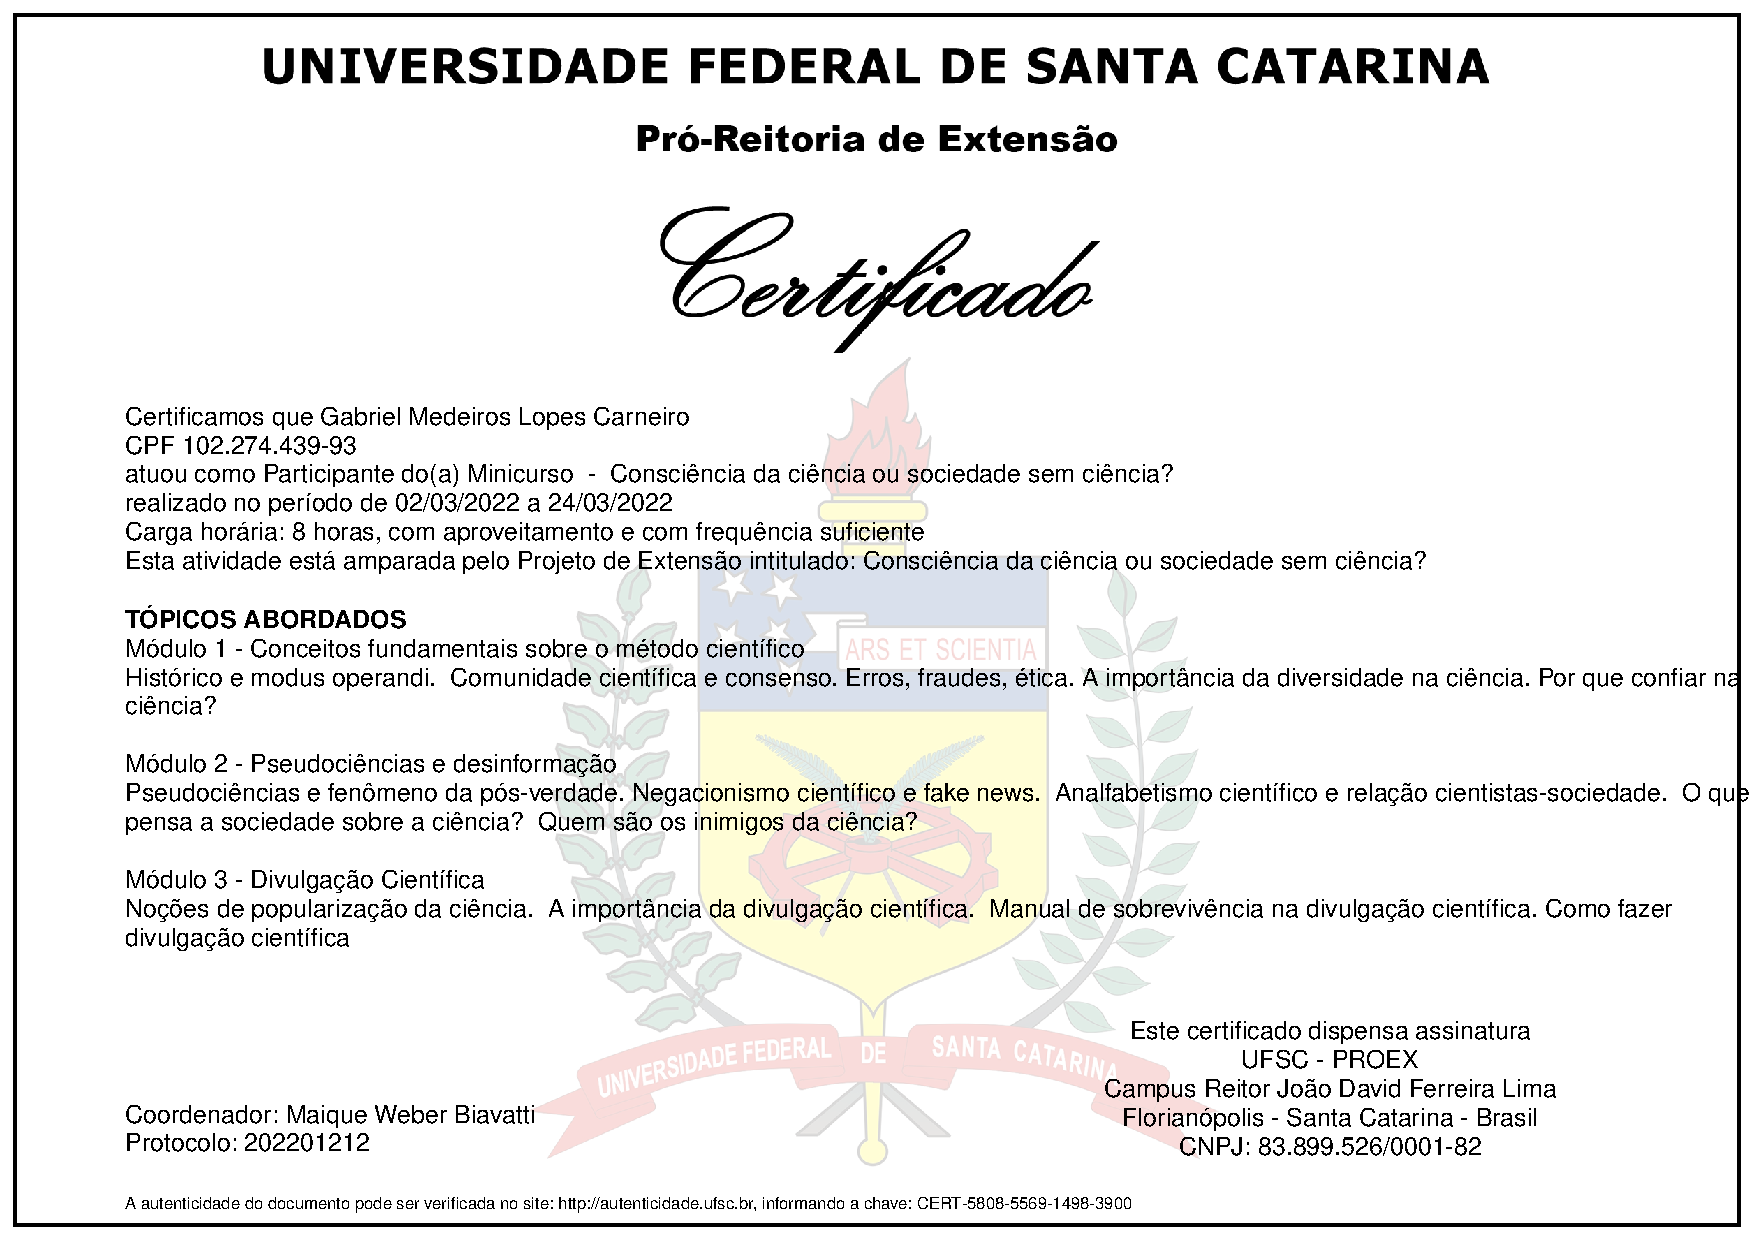
\includepdf{aftertext/minicurso-consciencia-ciencia}


\end{document}
% --------------------------------------------
% Final do documento. Não adicionar nada após.
% --------------------------------------------